Luego de diseñar el mapa de navegación para conocer el dominio de la aplicación se procede a estandarizar la interfaz de usuario, confeccionando la línea de diseño. Es por ello que en la \textbf{Figura \ref{fig: Linea_disenio}} se aprecia la posición de los elementos de la vista principal de la aplicación. En la parte superior se encuentra el encabezado y dentro de este último se ubica el logotipo, el botón de perfil de usuario, el botón de ayuda y el botón para cerrar sesión. Debajo del encabezado se encuentra el menú, donde van los íconos para que el usuario tenga el acceso a los distintos módulos de la aplicación. Luego se encuentra el contenido, el cual puede variar según la opción que el usuario seleccione en el menú. Por último, se puede observar el \emph{footer} (pié de página) de la aplicación.

\begin{figure}[h!tb]
    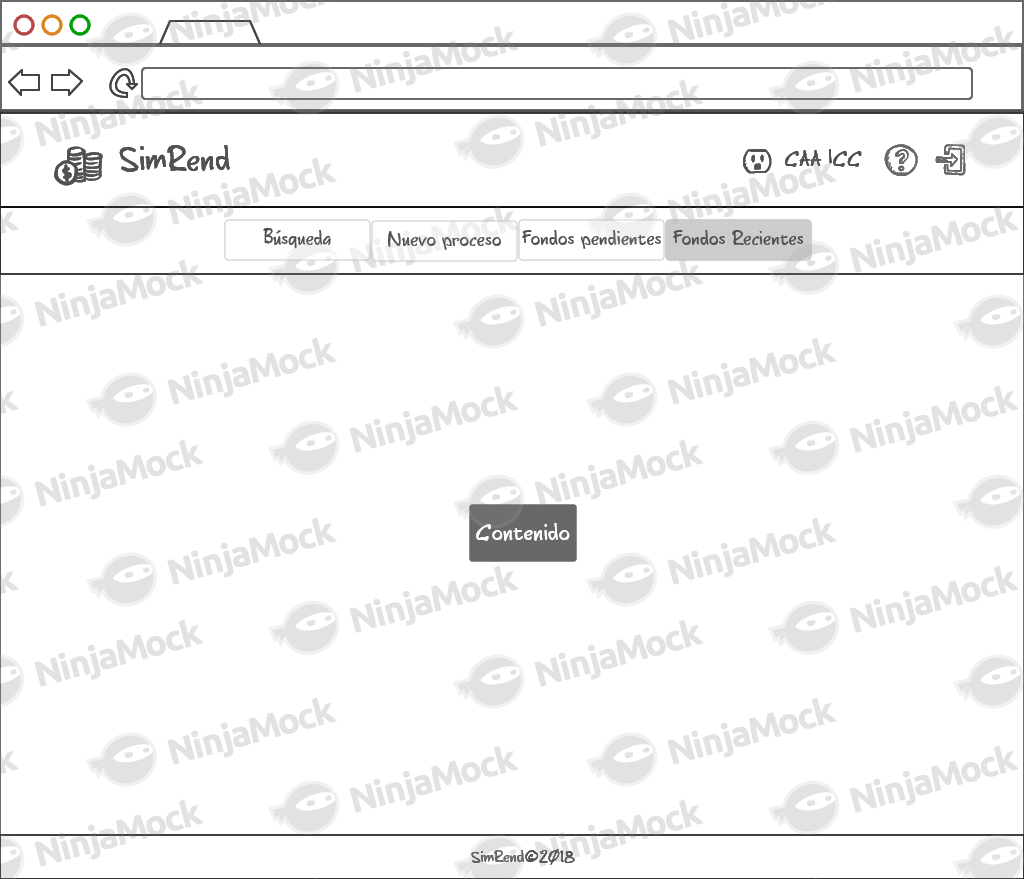
\includegraphics[width=\textwidth]{Imagenes/Linea_de_disenio.png}
    \caption{\label{fig: Linea_disenio}Línea de diseño de la aplicación que representa el estándar de los elementos de interfaz.}
\end{figure}